\documentclass[sigconf]{acmart}

\input{format/final}

\begin{document}


\title{Visualizing Crime in Los Angeles}

\author{Nishad Tupe}
\affiliation{%
  \institution{Indiana University}
  \streetaddress{Smith Research Center}
  

\city{Bloomington} 
  \state{IN} 
  \postcode{47408}
  \country{USA}}
\email{ntupe@iu.edu}

\author{Sushant Athaley}
\affiliation{%
  \institution{Indiana University}
  \streetaddress{Smith Research Center}
  \city{Bloomington} 
  

\state{IN} 
  \postcode{47408}
  \country{USA}}
\email{sathaley@iu.edu}

\author{Izolda Fetko}
\affiliation{%
  

\institution{Indiana University}
  \streetaddress{Smith Research Center}
  \city{Bloomington} 
  \state{IN} 
  

\postcode{47408}
  \country{USA}}
\email{ifetko@iu.edu}


\begin{abstract}

Crime and violence trace back to the 

beginning of human history. Our project utilizes publicly available data to analyze certain aspects of crime in 

the city of Los Angeles, California in the time period between January 2010 and September 2017. By visualizing 

those aspects, this project depicts certain trends that can be used to raise awareness among Los Angeles, 

California civic, and ultimately decrease crime rates in certain communities and city areas.

\end{abstract}

\keywords{Crime, Violence, Weapon, Victim, Crime scene, Visualization}

\maketitle

\section{Introduction}

Crime is 

one of the oldest social concepts and constructs. It stems from the early ages, with the beginning of the human 

interaction, and communication. According to the Merriam-Webster dictionary, crime is ``an illegal act for which 

someone can be punished by the government; especially: a gross violation of law'' \cite{www-merriam-webster}. 

Some acts and behaviors can be deemed unacceptable in some parts of the world while being celebrated by others. 

In both academic and public opinion, crime is usually associated with harm and violence and can be considered as 

one of the main problems that are affecting the quality of life and economic growth across the globe. In the 

recent years, we have witnessed intense migrations from Africa and Middle East to Europe. According to the UN 

Refugee Agency records, 68.5 million people are currently displaced worldwide \cite{www-UNHCR}. Out of those, 57 

percent of refugees come from three countries - South Sudan, Afghanistan, and Syria. For those people, violence 

and crime were the main deciding factors for migrating across the continent. Police departments, agencies are 

looking for more advanced geographic information systems that use complex data mining techniques, in order to 

improve crime analytics, with the ultimate goal to better protect their communities. Instead of just reacting to 

crimes as they happen, the new technology assists crime analysts to predict occurrence of events based on certain 

patterns and allows law enforcement to be proactive. According to Goldsmith's article from 2014, California 

public safety officials in Los Angeles are applying lessons and practices learned from earthquake predicting to 

preventing crime \cite{www-datasmart}.

In our project, we have been fostering similar ideas while visualizing 

crime data for the city of Los Angeles, California, in the time period between January 2010 and September 2017. 

Through our visualizations, we have tried to represent which types of crimes are most common, which demographic 

is most frequently targeted as victims, types of weapons used most frequently in certain crimes, along with the 

geographical areas most affected by certain types of crime. The result of this solution could be used to raise 

general awareness and help residents of Los Angeles identify dangerous locations and communities. It may also 

help recognize certain patterns and allow residents to be proactive by establishing non-profit organizations to 

educate young adults on violence and crime prevention. Moreover, it would allow the law enforcement agencies to 

develop strategies and ultimately reduce crime rates.

\section{Literature Review}

A large amount of work in regard 

to crime analysis and visualization has already been done. Large datasets have been reviewed, and information 

such as location and type of crimes have been extracted to help people follow law enforcements. Existing methods 

have used these databases to identify crime hotspots based on locations. In their paper, Almanie, Mirza, and Lor 

from University of Colorado, Boulder \cite{crime-prediction} focus on finding spatial and temporal criminal 

hotspots. They analyze two different real-world crime datasets for Denver, CO and Los Angeles, CA and provide a 

comparison between the two through a statistical analysis supported by several graphs. They also use A priori 

algorithm to produce interesting, frequent patterns of criminal hotspots, along with the decision tree, and a 

Naive Bayesian classifier in order to predict the potential crime types.

A different paper written by Spencer 

Chaney \cite{www-ucl} talks about the hypothesis testing processes for crime datasets. In his work, he describes 

the process of building the hypothesis, steps taken, and the case study example ``The overall process emphasis on 

'why' problem exist''. 

Unfortunately, not all crimes get reported to the Los Angeles Police Department (LAPD). A 

group of researchers, Arulanandam, Savarimuthu, and Purvis \cite{Arulanandam:2014:ECI:2667702.2667706}, focus on 

automatic extractions of public yet hidden information (available in the newspapers) and make it available to the 

general public. In their work, the emphasis is on theft crime and use of a CRF-based classifier model that is 

trained to identify crime locations from a set of articles. It also compares accuracy of identifying crime 

location in text by using the developed model on news articles from two other countries (Australia and India).

\section{Dataset Description}

We are collecting our data from various online public dataset repositories intended 

for public use. This dataset was originally released by the city of Los Angeles, California. Thus, provides us 

with an opportunity to use the data-driven analysis on various crime scenes in the city of Los Angeles. As 

mentioned on the website, ``the dataset was transcribed from original crime reports that are typed on papers'', 

hence, there might be some inaccuracies within data \cite{www-data-lacity}. The dataset along with the metadata, 

consist of different crime incidents reported or occurred between January 2010 and September 2017 \cite{www-

data-gov}. By performing different analysis and using visualization techniques learned in the Data Visualization 

class, we will be visualizing insights gained from crime incidents such as Victims Age Ranges, Victim 

Classification by Gender, Crime Area Geospatial Plots, Time Series Analysis, Top 10 crimes, and many others.


\section{Research Design and Methods}

This study will utilize crime dataset to analyze and visualize crimes 

pattern as follows but not limited to:
\begin{itemize}
\item Yearly crime rate
\item Month of the year with most 

crimes
\item Time of the day prone to crime
\item Geographical mapping of crime
\item Crime victim categorization by 

age, sex and descent
\item Weapons used in crime
\item Type of crimes
\item Crime investigation status and type of 

crime

\end{itemize}

We have used the methodology as shown in the process diagram (Figure \ref{f:meyhodology}) to 

conduct our study and publish the results.
\begin{figure}[!ht]
  \centering\includegraphics[width=\columnwidth]

{images/methodology.png}
  \caption{Methodology}\label{f:meyhodology}
\end{figure}

The first step included 

identifying the data source. Once we had established the data source, we had moved on to collection and data 

extraction. The following step included data load into Jupyter Notebooks using Python. The fourth step 

encompassed in data enhancement and clean-up, followed by data analysis and visualization. Once the 

visualizations were completed, we had used those polished results and published them.

Data Visualizations that let 

you discover trends or patterns in a data set are called Exploratory Data analysis. Before beginning the 

analysis, it is important to extract and clean the data. We used Python date time library and its methods to get 

the date, year, month columns. We also extracted latitude and longitude coordinates for Geo mapping from the 

location column. Once the data is in good shape, it is easier to gain the understanding of the data and 

visualization often becomes handy tool to find the interesting patterns. 

\subsection{Technologies}
Technologies 

and tools used in this project are:
\begin{itemize}
\item Python version 3.6, Jupiter Notebook
\item Matplotlib, 

Seaborn, Bokeh, Datashader, Holoviews, Googlemaps for visualization
\item Tableau 10.5
\end{itemize}

\subsection

{Code Organization}
Code is checked-in on GitHub at location \\
https://github.com/nishadtupe/DV-Project-SU-2018 \

\
Our code is organized as described in Figure \ref{c:code-structure}.
\begin{figure}[htb]
\begin{verbatim}
bin
 - 

Data_Clean_Categorical_Analysis.ipynb 
 - Time_Series_Analysis.ipynb
 - Geo_Mapping_Analysis.ipynb
data
   - 

Cleaned_Crime_Data.csv
   - Crime_Data_2010_2017.csv
\end{verbatim}
\caption{Code Structure}\label{c:code-

structure}
\end{figure}


\section{Visualizations and Observations}

\subsection{Time Series Analysis}

Time series 

analysis aims to understand patterns evolving over time and use those patterns to predict future behavior. This 

is especially useful in crime dataset analysis where each record has a timestamp value associated with it. If we 

look at the data year over year (Figure \ref{f:crime_by_year}), we can notice that overall, the number of crimes 

occurred and reported in Los Angeles, CA has significantly decreased. Moreover, it can be noticed that the 

relationship between reported and occurred crimes has changed over the years, having more crimes reported than 

occurred in 2010, an opposite relationship in the following years, up until 2015 where the number of crimes 

occurred and reported are coming to a single point. From 2015, we can notice a trend of fairly equal number of 

crimes occurred and reported, to finally see a small advantage in reported crimes in 2017. There is a negative 

trend in overall crime, but this could be little misleading since the data was collected until September of 2017. 

However, even if we remove year 2017 from the graph,  the crime rate would still be apparent.
\begin{figure}[!ht]
  

\centering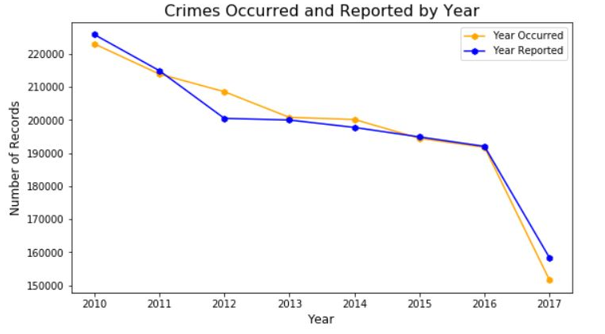
\includegraphics[width=\columnwidth]{images/crime_by_year.PNG}
  \caption{Crimes Occurred and Reported 

by Year}\label{f:crime_by_year}
\end{figure}

In Figure \ref{f:crime_by_month}, the fluctuation in number of crimes 

occurred by month can be noticed. This chart shows high crime rate from April to August. This can be loosely 

correlated to the fact that school vacations and people travel preferences are higher in this period, which 

eventually creates more opportunities for crime to occur. February and winter months (November and December) tend 

to have much lower crime counts.
\begin{figure}[!ht]
  \centering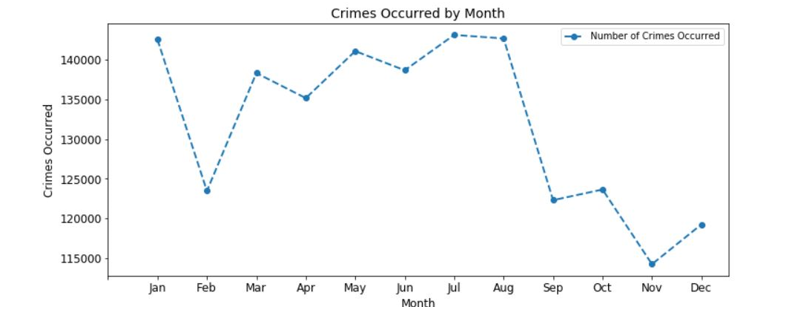
\includegraphics[width=\columnwidth]

{images/crime_by_month.PNG}
  \caption{Crime Number by Month}\label{f:crime_by_month}
\end{figure}

As shown in 

Figure \ref{f:Delta}, we can see the difference between crimes occurred to crimes reported. While it is not 

possible to report all crimes at actual time there is certainly room for improvement to reduce the delta. 
\begin

{figure}[!ht]
  \centering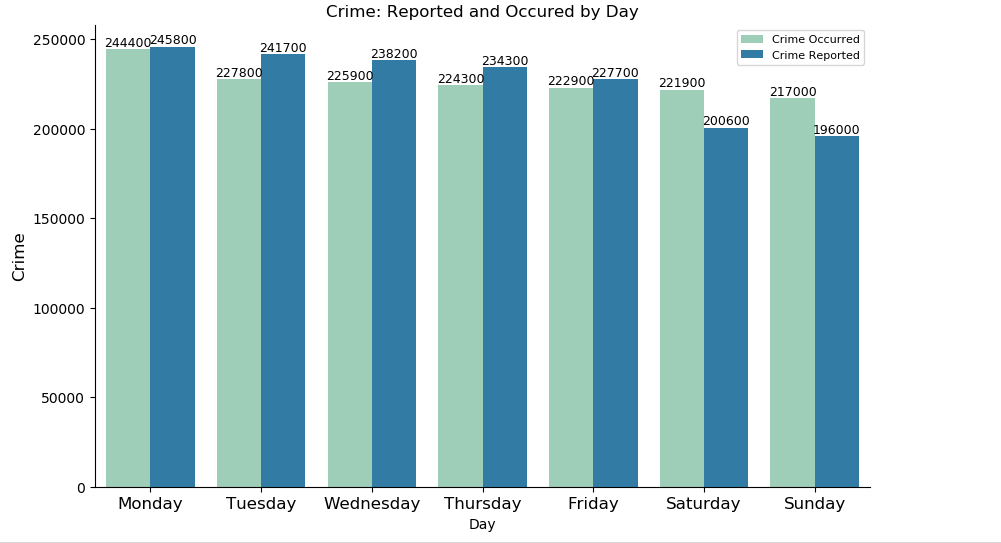
\includegraphics[width=\columnwidth]{images/Delta.PNG}
  \caption{Crime Reported and 

Occurred by Day}\label{f:Delta}
\end{figure} 

Victim sex analysis suggests that male side of the Los Angeles, CA 

public is more prone to become victims of crimes. This can be seen also from Figure \ref

{f:crime_by_victim_sex_year}, where the breakdown shows the number of victims by sex for each year. The ratio of 

male and female victims seems to be constant over the years, while the number of victims with unknown sex starts 

increasing in 2013 and reaching the highest value in 2016.
\begin{figure}[!ht]
  \centering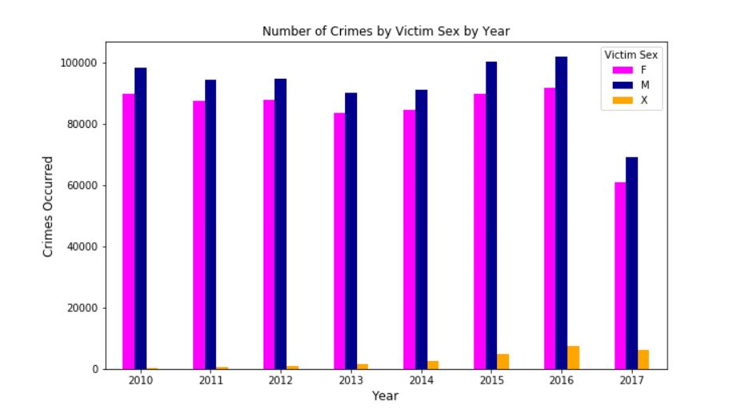
\includegraphics[width=

\columnwidth]{images/crime_by_victim_sex_year.PNG}
  \caption{Crimes by Victim Sex by Year}\label

{f:crime_by_victim_sex_year}
\end{figure}

Knowing the victim sex can tell us a lot about the crime, but additional 

information about their descent can help identify other motives of crime. In Figure \ref{f:victim_decsents}, we 

show the number of crimes occurred by victim descent. The highest number of victims in Los Angeles, CA are of 

Hispanic descent, followed by Caucasian and African-American. This may not indicate that there is some type of 

retaliation going on against the Hispanic residents, but that the majority of residents in Los Angeles may be of 

Hispanic descent.
\begin{figure}[!ht]
  \centering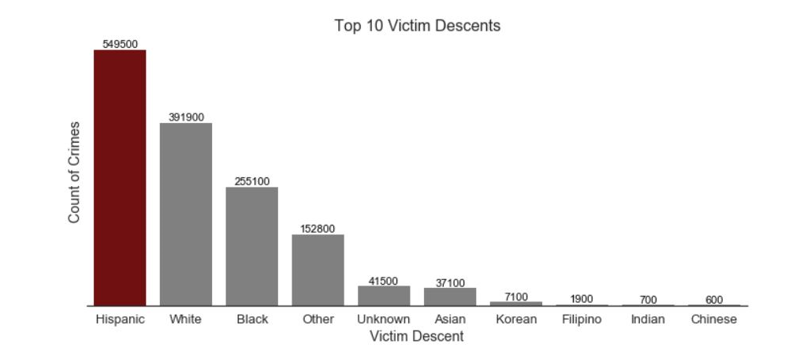
\includegraphics[width=\columnwidth]{images/victim_descents.PNG}
  

\caption{Top 10 Victim Decsents}\label{f:victim_decsents}
\end{figure}

If we break down the data even further as 

shown in Figure \ref{f:crime_victim_sex_hour}, by the hour of day, we can notice that majority of crimes for both 

male and female victims happen in early afternoon, while the number of crimes is pretty low in the early hours 

around 5am and 6am. An interesting fact that there a very intense spike in the hours between 11:30am and 2:00pm 

for both male and female victims.
\begin{figure}[!ht]
  \centering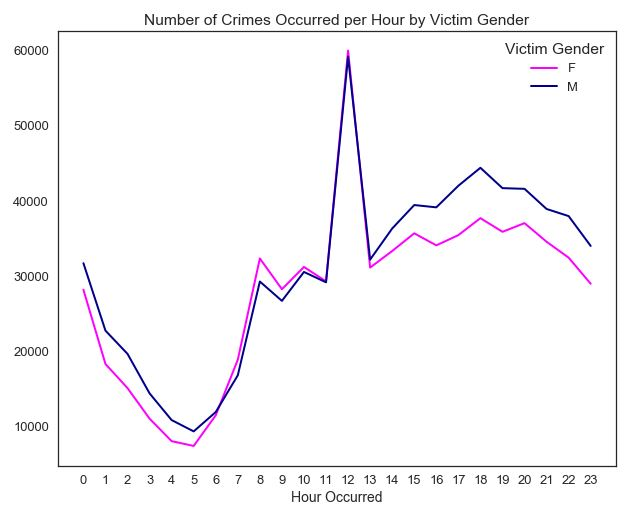
\includegraphics[width=\columnwidth]

{images/crime_by_victime_sex_hour.PNG}
  \caption{Crime by Victim Sex by Hour}\label{f:crime_victim_sex_hour}
\end

{figure}

\subsection{Statistical analysis}

Our statistical analysis was started with Histograms for continuous 

variable columns in the dataset. Our dataset contains only one numerical column, which  is the victims age. As 

Histograms are great at showing outliers and displaying how the data is distributed, we created a distplot 

(Figure \ref{f:Victim_Age_Distplot} ), where it can be seen that the probability of being a victim is higher for 

young people age between 25-40.
\begin{figure}[!ht]
  \centering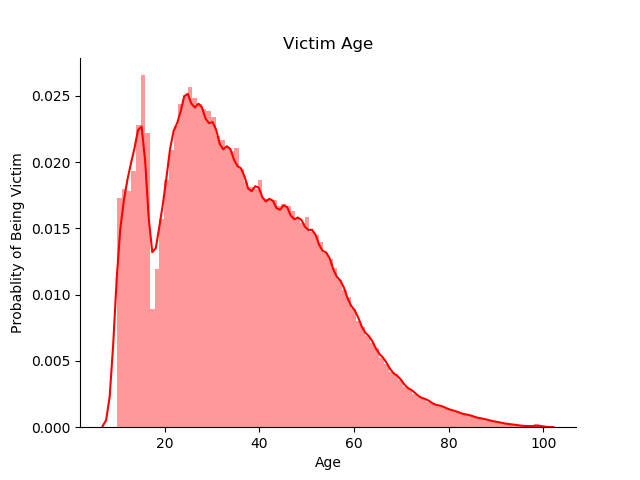
\includegraphics[width=\columnwidth]

{images/Victim_Age_Distplot.PNG}
  \caption{Victim Age Distplot}\label{f:Victim_Age_Distplot}
\end{figure}

The 

distribution of ages over victim gender shown in Figure \ref{f:Victim_Age_Historgram} ,  shows a slightly higher 

number of women victims observed than males in the age group between 20 and 40 years.
\begin{figure}[!ht]
  

\centering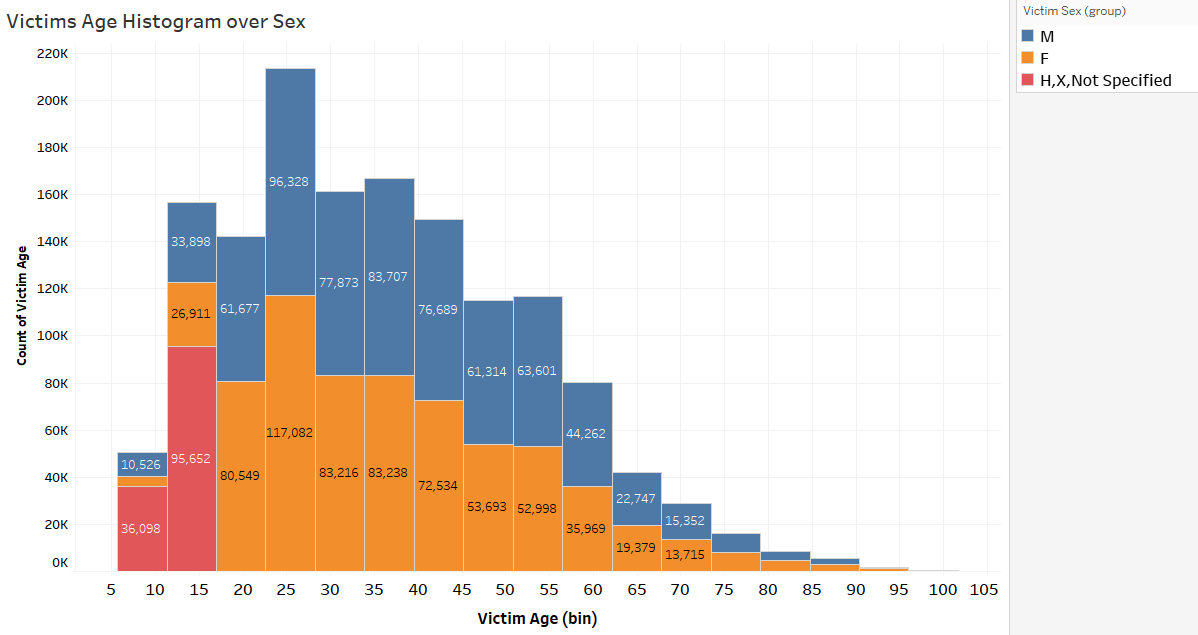
\includegraphics[width=\columnwidth]{images/Victim_Age_Historgram.PNG}
  \caption{Victims Age Over 

Sex}\label{f:Victim_Age_Historgram}
\end{figure} 

\subsection{Categorical Analysis}

With things like categorical 

variables, bar charts are ideal for comparing the categories. When comparing groups, bar charts are typically the 

best choice. We (humans) intuitively grasp differences based on the length and area of the bars. Bigger bars 

usually equal to more stuff. The focus of our project in this section was on top features in each category. 

Figure \ref{f:Top10_Crime_Types} shows the top 10 crime types such as Battery, Vehicle theft & Burglary which are 

among the highest rated crimes along with Vandalism, Intimate Partner (assault), and Cyber Crimes like Theft 

Identity. Crimes such as Drunk Roll, Train Wrecking, and illegal abortions are among the rare Crimes found in the 

dataset. Figure \ref{f:Top10_Crime_Areas} shows top areas where the crime took place, which fosters an important 

question. Are certain parts of Los Angeles more prone to crime than others? The answer is hidding in the Geo Maps 

visualizations. This is a perfect example that Geo Maps can be potentially used to validate Hypothesis. 
\begin

{figure}[!ht]
  \centering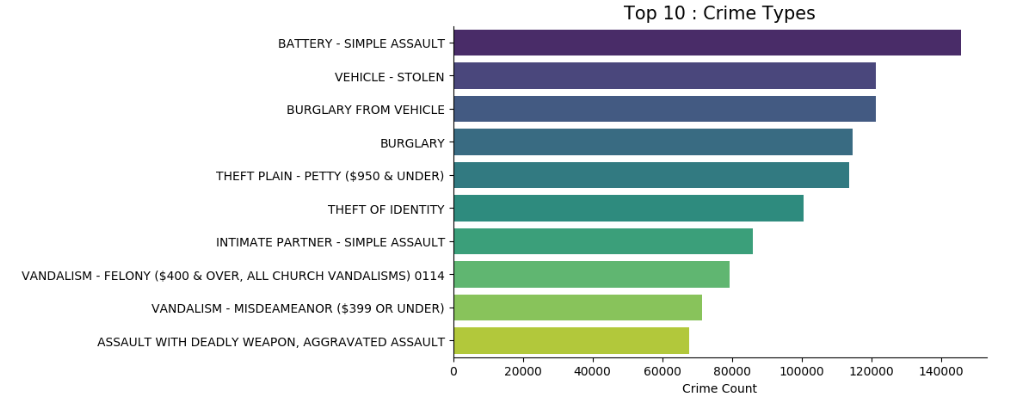
\includegraphics[width=\columnwidth]{images/Top10_Crime_Types.PNG}
  \caption{Top 10 

Crime Types}\label{f:Top10_Crime_Types}
\end{figure} 

\begin{figure}[!ht]
  \centering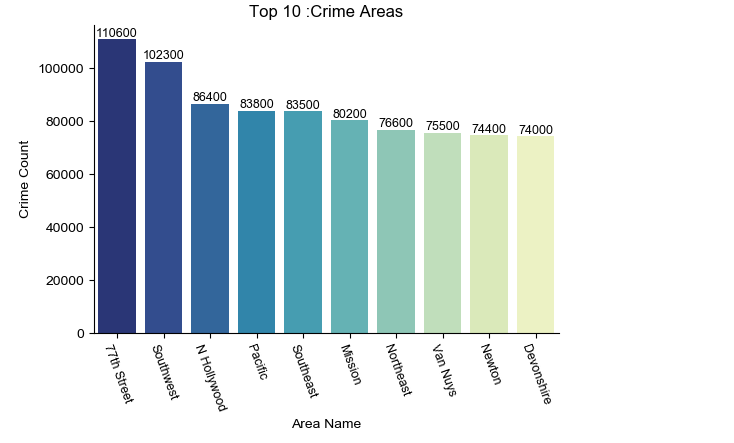
\includegraphics[width=

\columnwidth]{images/Top10_Crime_Areas.PNG}
  \caption{Top 10 Crime Spots}\label{f:Top10_Crime_Areas}
\end{figure}

Using the Seaborn factor plot, we had found that female victims have a higher probability of being victims of 

crimes related to the crime Code Descriptions such as Inmate Partner Assault and Battery Assault. This plot is 

shown in Figure \ref{f:crime_type_gender}.
\begin{figure}[!ht]
  \centering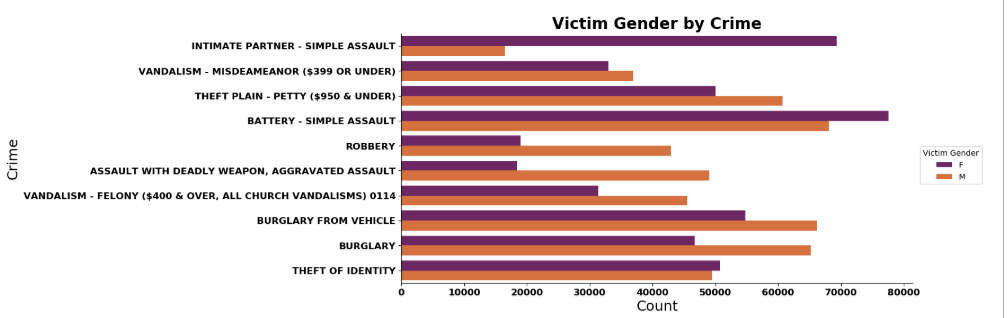
\includegraphics[width=\columnwidth]

{images/Crime_By_Victim_Gender.PNG}
  \caption{Crime Types and Gender}\label{f:crime_type_gender}
\end{figure}

\subsection{Geo-Spatial Analysis}
Crime location provides important information about the crime prone areas and 

can help us understand crime hot spots. Location information present in the dataset has been converted to 

separate columns as longitude and latitude to perform various Geo-spatial analysis. A joint plot is an important 

visualization technique which help us visualize bivariate and univariate distribution on the same plot. We plot 

locations in Figure \ref{f:crime_location_join} using hexagonal binning technique along with the histogram. This 

graph provides an idea about distribution of longitude and latitude along with the crime prone area. 
\begin

{figure}[!ht]
  \centering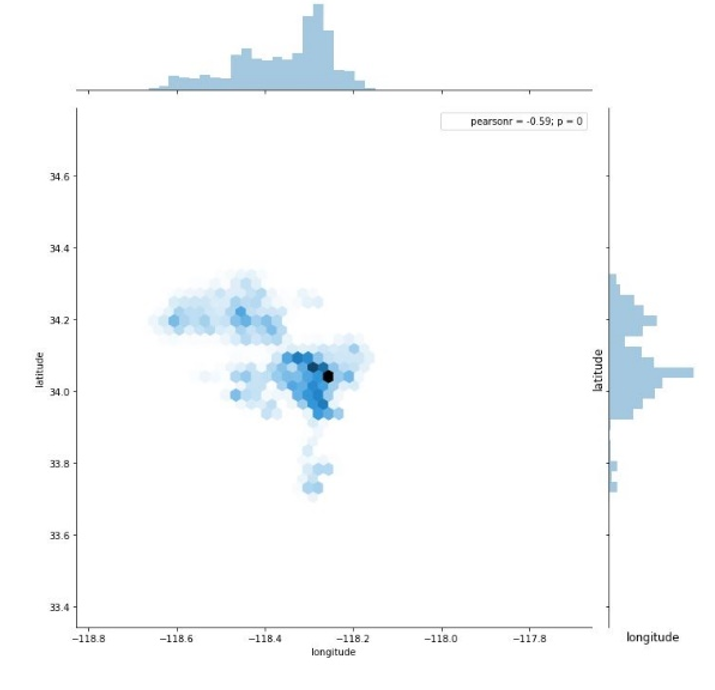
\includegraphics[width=\columnwidth]{images/location_joint_plot.PNG}
  \caption{Crime 

Location Distribution}\label{f:crime_location_join}
\end{figure}

We used Datashader available in Python to plot a 

nice heat map of the crime location in Figure \ref{f:crime_location_heatmap}. This plot doesn't provide exact 

location of the crime in terms of area on the map but it still provides a nice visualization of the impacted 

area.
\begin{figure}[!ht]
  \centering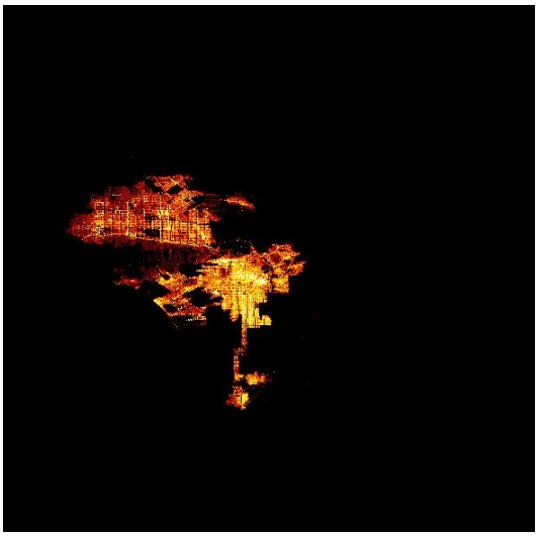
\includegraphics[width=\columnwidth]{images/heat_map.PNG}
  \caption{Crime 

Location Heat Map}\label{f:crime_location_heatmap}
\end{figure}

To get the exact locations of crime, we used Google 

maps along with the Bokeh library. Google map provides area names and Bokeh provides us with interactive tools 

like zoom in and zoom out. Figure \ref{f:crime_location_google} shows crime locations in red on Google Map along 

with the area names. This map helped us identify areas in Los Angeles where crime has happened,and to show that 

crime is mostly concentrated in the city center area. Adding surveillance or taking precautions as well as 

avoiding this area during night times can be used as a preventive measure to reduce crime.
\begin{figure}[!ht]
  

\centering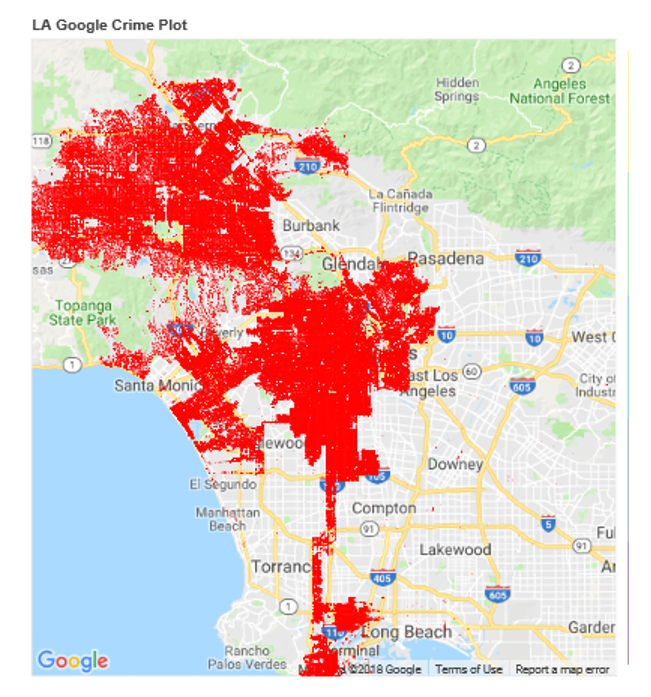
\includegraphics[width=\columnwidth]{images/google_plot_al.PNG}
  \caption{LA Crimes Google Map}\label

{f:crime_location_google}
\end{figure}

\subsection{Text Analysis}

In order to get more insights related to the Los 

Angeles crime activities, we had conducted a text analysis of our data. We applied the world cloud visualization 

on the crime premise information to understand the specific places where the crimes occur. As shown in Figure 

\ref{f:Top_Premises} , the top premises where crime has occurred includes street, family dwelling places, and 

parking lots. We used the total of percentile table calculation to conclude that more than 50\% of the highly 

rated crimes take place above premises.
\begin{figure}[!ht]
  \centering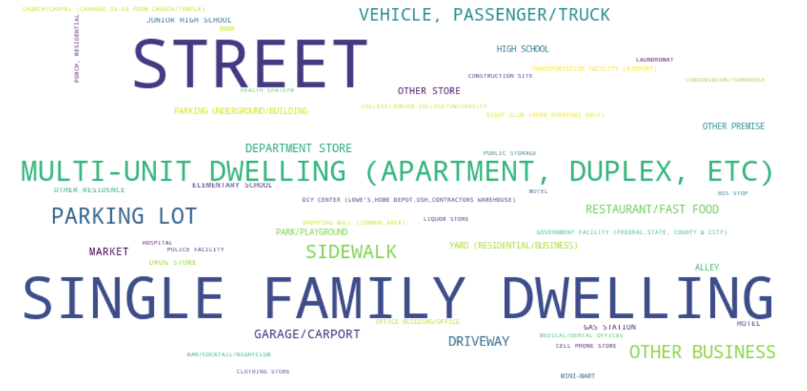
\includegraphics[width=\columnwidth]

{images/Top_Premises.PNG}
  \caption{Word Cloud - Top Premises}\label{f:Top_Premises}
\end{figure}

\subsection{Other 

Interesting Visualizations}

We analyzed the weapon used to commit crime data by using a bubble chart. Tableau 

Bubble Chart displays the data in circles. The tool had allowed us to define each bubble by using any of the 

dimension members and its size by using a measure value. Figure \ref{f:word_cloud_crime_type} shows that arms or 

body force is the most used weapon to commit crime, followed by verbal threat. This also suggests that most of 

the crimes are not planned but are crimes of passion and instantaneous reactions.
 \begin{figure}[!ht]
  

\centering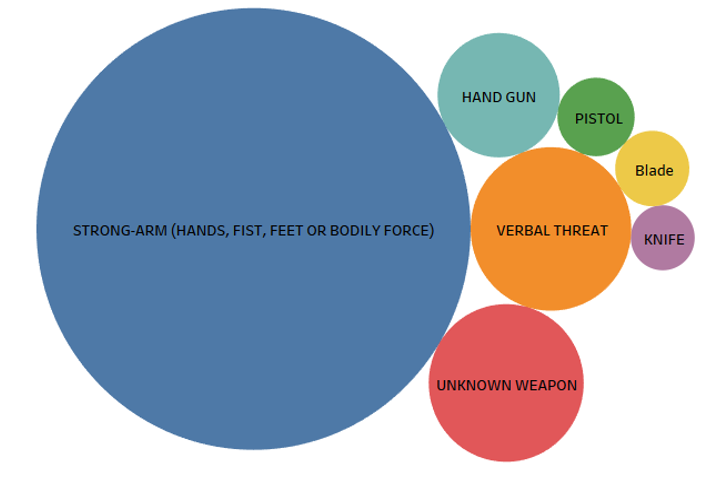
\includegraphics[width=\columnwidth]{images/bubble.PNG}
  \caption{Crime - Weapons Used}\label

{f:word_cloud_crime_type}
\end{figure}

The visualization in Figure \ref{f:Confusion_Matrix} shows correlation 

between crime types. Shoplifting and petty theft are highly correlated.
\begin{figure}[!ht]
  \centering

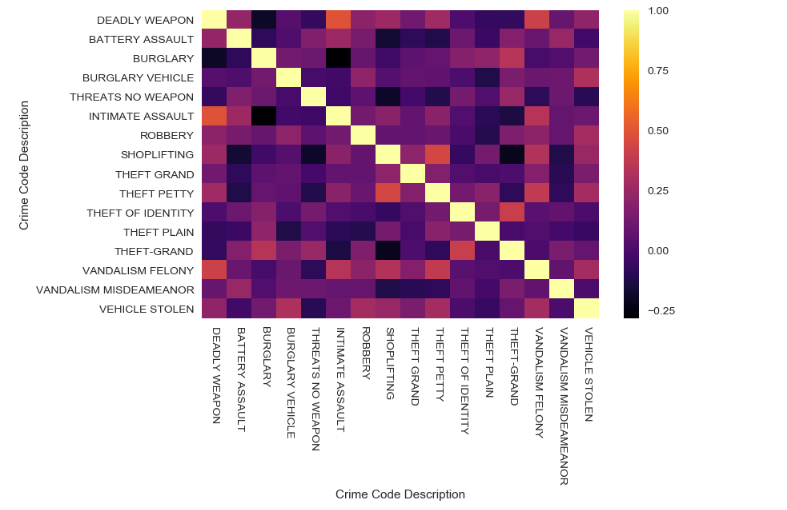
\includegraphics[width=\columnwidth]{images/Confusion_Matrix.png}
  \caption{Correlation Matrix}\label

{f:Confusion_Matrix}
\end{figure}

\section{Conclusion}

Although a significant crime rate decrease has been recorded 

(27\%) in the Los Angeles city area since 2010, the modern society still has a long way to go until crime rates 

reach acceptable levels. Our research had found that individuals should take caution when visiting downtown 

areas, especially the 77th Street in warmer months, as crime tends to peak during those times. Stand-alone houses 

and vehicles, as well as younger male individuals age 25-40 are frequently targeted by criminals, so city 

residents and visitors should keep this in mind when entering and exiting their residences, and moving around in 

the area. Moreover, high crime area residents should consider incorporating security systems into their homes and 

vehicles. Another great example for residents on how to increase security in these areas is to increase 

surveillance through neighborhood watch. When it comes to the Los Angeles law enforcement, we recommend increased 

patrol routes in the downtown areas in mid-day and mid-night, as frequent crime occurrence has been linked to 

these time-frames. In addition to the increased patrolling, we recommend establishing youth groups in the 

affected areas where the law enforcement officers would share their experiences, raise awareness, and educate 

young individuals on how to report suspicious activity and other crime prevention techniques. In our research, we 

have also found that data visualization not only  provides exploratory data analysis but also helps us understand 

kind of measures we may want to take in order to reduce crime rates and make our cities safer while saving human 

lives.

\begin{acks}

  The authors would like to thank the Data Visualization course teaching staff, mainly 

professor Y. Y. Ahn for their support and guidance during this project. Also, we would also like to extend our 

appreciation to Kaggle for providing us with the Los Angeles Crime dataset, and to other online sources for 

allowing us to gather meaningful insights and programming support

\end{acks}

\bibliographystyle{ACM-Reference-

Format}
\bibliography{report} 

\appendix

%\input{issues}

\end{document}
